


\section{Experiments}

In this section, we first study the effectiveness of multi-token entropy decoding for parallel sampling. Then, we examine the inference-time and post-training benefits of {reasoning-as-infilling}, such as (1) early-exits based on answer certainty $H_\textsc{ub}(\mba \mid \mbr_{\textsc{un-masked}}, \mbc)$ and (2) the ability to bootstrap and score reasoning traces given (question, answer) pairs. 

\subsection{Accelerated sampling with Multi-token Entropy Decoding}

In this experiment, we show that entropy-thresholded multi-token decoding (\textsc{med}) enables parallel decoding without incurring the distributional error and performance degradation that fixed multi-token decoding incurs. 

For these experiments, we use two open-source \glspl{mdlm} models, Dream-7B Instruct \citep{dream2025} and LLaDA-8B Instruct \citep{nie2025largelanguagediffusionmodels}. We consider two popular benchmarks, (1) \textsc{gsm8}k \citep{lightman2023letsverifystepstep}, a mathematical reasoning dataset, and (2) HumanEval \citep{chen2021evaluating}, a coding benchmark. As baselines, we consider the entropy decoding scheme $\sigma_{\textsc{entropy},k}$ \citep{chang2022maskgit,ye2025dream}, which decodes a fixed number of $k$ tokens in each step. We consider $k \in \{1, 2\}$. 

For evaluations, we measure the task accuracy and the number of function evaluations (\textsc{nfe}s) for varying values of $k$ in the fixed token decoding scheme as well as varying values of $\lambda \in \{0.1, 0.2, 0.3\}$ in \gls{med} with $k_{\text{max}}=32$ as the maximum number of tokens decoded in parallel. We fix a generation length $L = 128$ and a block size of $32$. 

\begin{figure*}[t]
    \centering
    \begin{minipage}[c]{0.58\textwidth}
        \centering
        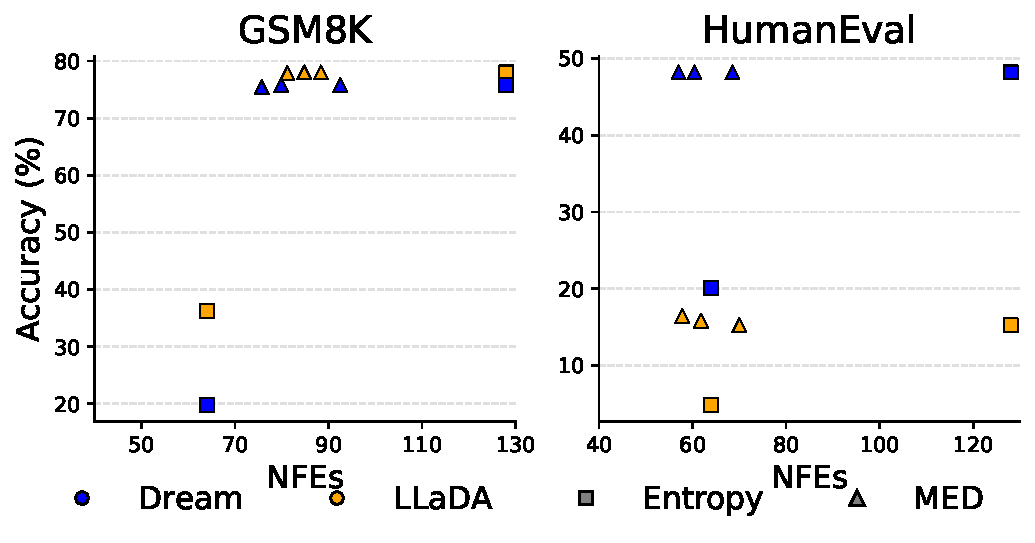
\includegraphics[width=\linewidth]{plots/performance_scatter_kdash_dynamicx20.pdf}
    \end{minipage}%
    \hfill
    \begin{minipage}[c]{0.38\textwidth}
        \caption{\textbf{\gls{med} enables parallel token decoding without any loss in performance.}
        We compare \gls{med} decoding with $\lambda \in \{0.1, 0.2, 0.3\}$ to entropy decoding
        with a fixed number of tokens $k \in \{1, 2\}$.
        We observe that \gls{med} significantly reduces the number of NFEs
        while matching accuracy and maintaining a low KL.}
        \label{fig:multi_token_kl}
    \end{minipage}
\end{figure*}

In \cref{fig:multi_token_kl}, we observe:
\begin{itemize}[leftmargin=*]
    \item Decoding just $k=2$ tokens in parallel results in a large drop in accuracy on \textsc{gsm8}k for both LLaDA and Dream ($>40\%$). We observe that decoding $k=2$ also leads to a significant increase in \gls{kl}. 
    \item \gls{med} with $\lambda=0.2$, provides significant speed-ups and \textit{no loss in accuracy} for both LLaDA and Dream. For \textsc{HumanEval}, \gls{med} results in identical accuracy with a $2.2\times$ speed-up, and on \textsc{gsm8}k, we observe a $1.5\times$ speed-up with no loss in performance. 
\end{itemize}

Additionally, in \cref{tab:multi_token_kl}, we also measure the \gls{kl} divergence between the likelihoods of the single-token decoding scheme with the multi-token decoding schemes. The likelihood for each decoding scheme $\sigma = (\sigma_1, \sigma_2, \dots, \sigma_n)$ is computed as $\prod_{t=1}^{n} p_\theta(x_{\sigma_t} \mid \mbc, \mbx_{\sigma_{<t}})$ where $n \leq t$ and $\sigma_t$ denotes the position(s) decoded at step $t$. When decoding multiple tokens in a single step, we use the conditionally independent factorization. In contrast to fixed decoding with $k=2$ tokens, the \gls{kl} divergence between \gls{med} and single-token entropy decoding is substantially lower even with fewer \textsc{nfe}s, and scaling $\lambda$ offers a trade-off between fewer \textsc{nfe}s and \textsc{kl}.

    
\subsection{The benefits of {reasoning-as-infilling}}
\paragraph{Early exits.} We investigate the inference-time benefits of {reasoning-as-infilling} on two mathematical reasoning datasets, \textsc{gsm8}k \citep{lightman2023letsverifystepstep} and \textsc{math500} \citep{cobbe2021training}, with the Dream 7B and LLaDA-8B models. 

For both tasks, we consider a generation length $L = 256$ with block size 32. We pre-fill the answer delimiter \textit{``The answer is \textbackslash boxed\{.."}, and allocate $10$ answer tokens. As a baseline, we compare against allocating a sequence of length $256$ with no-reasoning template. For sampling, we examine early exits with one-token decoding and both \gls{med} and \textsc{ar-med} with $\lambda = 0.2$. 

In \cref{tab:early_exit_combined}, we observe:
\begin{itemize}[leftmargin=*]
    \item For both Dream and LLaDA, early exiting reduces the total number of \textsc{nfe}s, and increasing the early exit threshold $\gamma$ enables trading faster inference for task accuracy. For example, for LLaDA, we observe a $23\%$ speed up on one-token entropy decoding with only a  $<1\%$ drop in performance versus baseline reasoning template. Early exits combined with \gls{med} and \textsc{ar-med} provide further savings.  LLaDa with \gls{med} and $\gamma=0.1$ outperforms the base configuration on \textsc{gsm8}k with a $3.3\times$ speedup.

    \item Notably, the benefits of early exits are more pronounced for LLaDA than Dream, which requires higher exit thresholds for speed-ups. This may be due to Dream's adaption from an \gls{ntp} model \citep{gong2024scaling,dream2025}. See \cref{appsec:observations} for a discussion of the sampling behavior of Dream and LLaDA. 
\end{itemize}


\begin{table}[h]
    \centering
    \begin{tabular}{ll ccc ccc}
\toprule
\multicolumn{2}{c}{} & \multicolumn{3}{c}{\textbf{GSM8K}} & \multicolumn{3}{c}{\textbf{Math500}} \\
\cmidrule(lr){3-5} \cmidrule(lr){6-8}
\textbf{Model} & \textbf{Sampler} & \textbf{Exit Param} & \textbf{NFEs} $\downarrow$ & \textbf{Acc.} $\uparrow$ & \textbf{Exit Param} & \textbf{NFEs} $\downarrow$ & \textbf{Acc.} $\uparrow$ \\
\midrule
        LLaDA & $\sigma_{\textsc{entropy}, k=1}$ & \textsc{no template} & 256 & 76.6 & \textsc{no template} & 256 & \textbf{33.8} \\
        LLaDA & $\sigma_{\textsc{entropy}, k=1}$ & \textsc{no exit}     & 256 & 79.4 & \textsc{no exit}     & 256 & 33.4 \\
        LLaDA & $\sigma_{\textsc{entropy}, k=1}$ & $\gamma=0.1$         & 193 & 78.6 & $\gamma=0.3$         & 221 & 31.9 \\
        \midrule
        LLaDA & $\sigma_{\gls{med}, \lambda = 0.2}$ & \textsc{no exit}   & 94  & \textbf{79.9} & \textsc{no exit}   & 143 & 33.4 \\
        LLaDA & $\sigma_{\gls{med}, \lambda = 0.2}$ & $\gamma=0.1$       & \textbf{77}  & 79.3 & $\gamma=0.3$       & 129 & 32.0 \\
        \midrule
        LLaDA & $\sigma_{\textsc{ar-med}, \lambda = 0.2}$ & \textsc{no exit} & 105 & 79.2 & \textsc{no exit} & 143 & 33.4 \\
        LLaDA & $\sigma_{\textsc{ar-med}, \lambda = 0.2}$ & $\gamma=0.1$     & 93  & 78.1 & $\gamma=0.3$     & \textbf{128} & 31.7 \\
        \midrule\midrule
        Dream & $\sigma_{\textsc{entropy}, k=1}$ & \textsc{no template} & 256 & \textbf{80.1} & \textsc{no template} & 256 & 33.4 \\
        Dream & $\sigma_{\textsc{entropy}, k=1}$ & \textsc{no exit}     & 256 & 79.8 & \textsc{no exit}     & 256 & \textbf{35.6} \\
        Dream & $\sigma_{\textsc{entropy}, k=1}$ & $\gamma=0.7$         & 225 & 76.7 & $\gamma=0.7$         & 245 & 33.2 \\
        \midrule
        Dream & $\sigma_{\gls{med}, \lambda = 0.2}$ & \textsc{no exit}   & 135 & 79.2 & \textsc{no exit}   & 147 & 35.6 \\
        Dream & $\sigma_{\gls{med}, \lambda = 0.2}$ & $\gamma=0.7$       & \textbf{121} & 79.3 & $\gamma=0.7$       & 141 & 35.4 \\
        \midrule
        Dream & $\sigma_{\textsc{ar-med}, \lambda = 0.2}$ & \textsc{no exit} & 148 & 77.1 & \textsc{no exit} & 151 & 35.6 \\
        Dream & $\sigma_{\textsc{ar-med}, \lambda = 0.2}$ & $\gamma=0.7$     & 131 & 73.9 & $\gamma=0.7$     & \textbf{136} & 35.0 \\
    \bottomrule
    \end{tabular}
    \caption{\textbf{Early-exits can accelerate \gls{mdlm} inference.} We evaluate reasoning-as-infilling with early exits on a generation length of $256$. Varying the early exit threshold $\gamma$ enables trading faster inference for task accuracy. Lower values of $\gamma$ preserve performance.}
    \label{tab:early_exit_combined}
\end{table}

Next, we investigate how a dataset of question-answer pairs $\{(\mbc_i, \mba_i)\}_{i=1}^{N}$, can be used to analyze and improve \glspl{mdlm}. 

\begin{table}[h]
\centering
\begin{tabular}{lcc}
\toprule
\textbf{Model} & \multicolumn{2}{c}{\textbf{Posterior Reasoning Scores}} \\
\cmidrule(lr){2-3}
 & \textbf{Qwen2.5-Math-PRM} & \textbf{GPT-4o} \\
\midrule
LLaDA-8B Base  & 0.31 & 0.36 \\
LLaDA-8B Instruct & 0.38 & 0.43 \\
\bottomrule
\end{tabular}
\label{tab:judge_scores}
\caption{\textbf{The \gls{mdlm} reasoning posterior yields high-quality traces for problems that the original instruct-tuned model fails to solve.} We perform posterior inference on the $1419$ training samples that LLaDa-8B Instruct with greedy decoding fails to solve, and evaluate the resulting traces with two judges, \textsc{Qwen2.5-Math-PRM} \citep{zhang2025lessons} and \textsc{gpt-4}o \citep{hurst2024gpt}. Both judges rate $\sim40\%$ of the instruct-tuned reasoning chains as correct. Notably, even the posterior reasoning chains from the base model are rated as $>31\%$ correct.}
\end{table}

\begin{table}[h]
\centering
\small
\begin{tabular}{lcc}
\toprule
\textbf{Model} & \textbf{Post-training Data} & \textbf{GSM8K Test Acc.} \\
\midrule
LLaDA 8B-Base (No reasoning template) & - & 13.9 \% \\
LLaDA 8B-Base (With reasoning template) & - & 51.2  \% \\
\midrule
Finetuned$^*$ LLaDA 8B-Base & \textsc{gsm8}k $(\mbc, \mbr_\text{gold}, \mba_\text{gold})$ ($n=7473$) & 64.6 (\textcolor{teal}{$+13.4$})  \% \\
Finetuned$^*$ LLaDA 8B-Base & \textsc{gsm8}k Posterior $(\mbc, \mbr_\text{posterior}, \mba_\text{gold})$ ($n=7473$) & {66.1} (\textcolor{teal}{$+14.9$})  \% \\
\midrule 
LLaDA-8B Instruct & Misc. Instruction Data ($n=4.5$ million) & 75.96  \% \\ 
\bottomrule
\end{tabular}
\caption{\textbf{Fine-tuning the base model with posterior-generated data improves performance.} 
Fine-tuning on \textsc{gsm8}k training data and posterior reasoning traces boosts accuracy to $64.6\%$ and $66.1\%$, respectively. Finetuned$^*$ indicates LoRA \citep{hu2022lora} fine-tuning.}
\label{tab:finetune_gsm8k}
\end{table}




\paragraph{The answer posterior is a source of high-quality reasoning traces.} 

Here, we evaluate reasoning traces $\mbr$ generated from the posterior distribution $p_\theta(\mbr \mid \mbc, \mba)$. A key challenge for training better reasoning models is collecting high quality reasoning traces \citep{zelikman2022star}. We investigate whether the  \gls{mdlm}  posterior distribution can provide these traces, even when an \gls{mdlm} incorrectly solves the original task.
To do this, we utilize question-answer pairs from \textsc{gsm8}k \citep{lightman2023letsverifystepstep}. In this experiment, we generate samples from the LLaDA-8B Instruct model with \gls{med} and any-order decoding. On the \textsc{gsm8}k training dataset, the model answers $1419$ out of $7473$ problems incorrectly. We use these $1419$ question-answer pairs to generate reasoning traces from the \gls{mdlm} posterior (i.e. with the answer pre-filled). We also generate reasoning traces with the base model (without instruction tuning).

To evaluate these reasoning traces for correctness, we use \textsc{gpt4}o \citep{hurst2024gpt}, and the Qwen2.5-Math-7B \textsc{prm} \citep{zhang2025lessons}, see \cref{appsec:gpt4_prompt} for the system instructions to the \textsc{gpt4}o model. In \cref{tab:judge_scores} observe that both judge models rate $\sim40\%$ of the posterior reasoning traces as correct. In \cref{appsec:posterior_traces}, we include examples of reasoning traces generated from the posterior and the regular model with different judge labels. We observe that the posterior traces judged correct by \textsc{gpt4}o contain accurate reasoning steps, correcting the original model's behavior. Notably, we also observe that {reasoning-as-infilling} elicits correct reasoning chains ($>30\%$) from the base model checkpoint on these problems. 







    


\paragraph{Posterior data can be used to improve base models.} Here, we examine the effectiveness of post-training on the post-hoc reasoning dataset generated on the full \textsc{gsm8}k training set with the base model. We post-train the LLaDA-8B Base model using LoRA \citep{hu2022lora}. 

In \cref{tab:finetune_gsm8k}, we observe that fine-tuning the model on the posterior generated base model data significantly improves performance ($+14.9\%$).
As a benchmark, we observe that fine-tuning on the \textsc{gsm8}k \textit{human annotated} reasoning traces produces similar results. These results provide evidence that maximizing the log-likelihood $\log p_\theta(\mba, \mbr \mid \mbc)$ on the posterior reasoning traces improves accuracy on reasoning tasks. We include additional training details \cref{appsec:finetuning}. 



\paragraph{Scoring partial reasoning traces without an external model.} 
\citet{zhang2024rest} show that using intermediate process rewards for sampling can improve model fine-tuning. However, training these process rewards requires training an external model. In \cref{fig:correct_correlations}, we compare various strategies for estimating the final correctness of partial reasoning traces given intermediate rewards. 

Using the LLaDA-8B Instruct model, we greedily sample solutions on the \textsc{gsm8}k test set, left-to-right, $1$ token at a time. We then compute the Pearson correlation between intermediate rewards and the correctness of the final output. During reasoning, the intermediate reasoning process defined using the answer log probabilities $\log p_\theta(a_j = a_j^* \mid \mbc, \mbr_{\textsc{un-masked}})$ are more strongly correlated with final answer correctness at intermediate steps than a pretrained 7B parameter process reward model \citep{zhang2025lessons}. 









Notably, we also find that measuring answer block log probabilities enables filtering lower-quality reasoning chains generated via posterior sampling. Given a posterior reasoning chain without the prefilled answer, the \gls{mdlm} mean answer probabilities can predict \textsc{gpt4}-o reasoning chain correctness scores, see \cref{appsec:posterior_filtering}.

Our results provide evidence that \gls{mdlm} pre-training offers other new post-training capabilities: low-quality reasoning chains could be terminated early or filtered, the reasoning process could be steered towards correct solutions, reflection tokens could be automatically inserted at reasoning failures, and new sources of dense feedback could incorporated into fine-tuning objectives.


\begin{figure}[t]
    \centering
    \begin{minipage}[c]{0.44\textwidth}
        \centering
        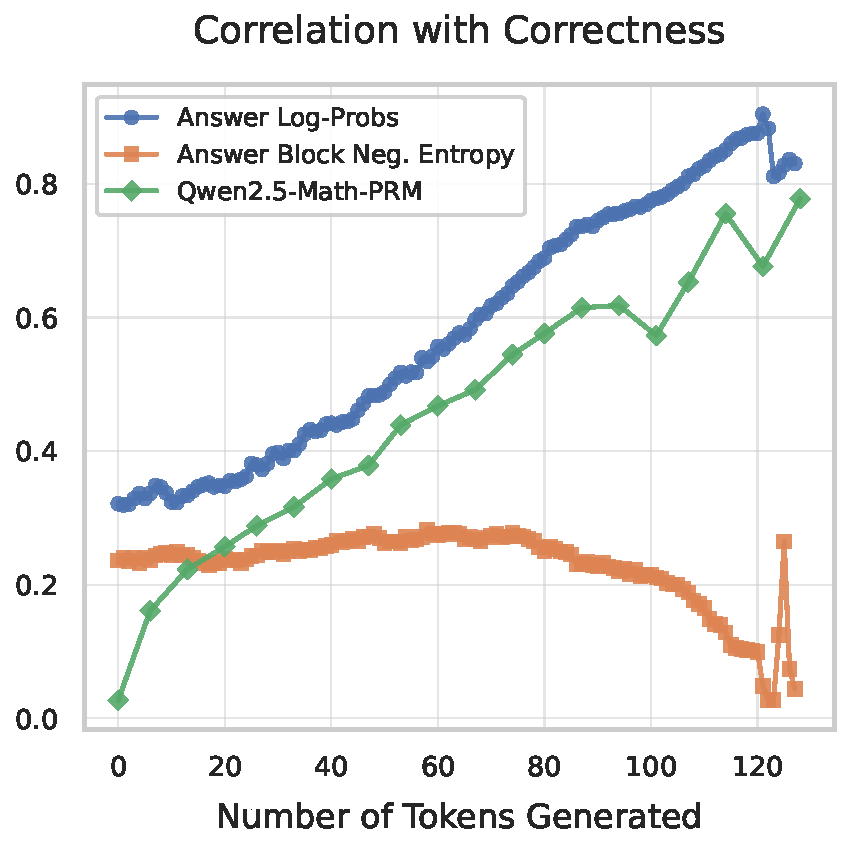
\includegraphics[width=\linewidth]{plots/correlations.pdf}
    \end{minipage}%
    \hfill
    \begin{minipage}[c]{0.44\textwidth}
        \caption{\textbf{\glspl{mdlm} enable scoring their own reasoning process without an external process verifier.}
        We score \textsc{gsm8}k reasoning traces, generated left-to-right with LLaDA, at intermediate steps using
        (a) gold answer log probabilities, (b) the answer block entropy bound, and (c) an 8B process reward model (PRM) \citep{zhang2025lessonsdevelopingprocessreward}.
        Gold answer probability at intermediate steps is more predictive of final correctness than PRM scores.
        Even without gold labels, the answer block entropy is weakly correlated with correctness.}
        \label{fig:correct_correlations}
    \end{minipage}
\end{figure}









